\documentclass[12pt,letterpaper,fleqn]{hmcpset}
\usepackage[margin=1in]{geometry}
\usepackage{graphicx}
\usepackage{amsmath,amssymb}
\usepackage{enumerate}
\usepackage{hyperref}
\usepackage{parskip}
\usepackage{listings}

% Theorems
\usepackage{amsthm}
\renewcommand\qedsymbol{$\blacksquare$}
\makeatletter
\@ifclassloaded{article}{
    \newtheorem{definition}{Definition}[section]
    \newtheorem{example}{Example}[section]
    \newtheorem{theorem}{Theorem}[section]
    \newtheorem{corollary}{Corollary}[theorem]
    \newtheorem{lemma}{Lemma}[theorem]
}{
}
\makeatother

% Random Stuff
\setlength\unitlength{1mm}

\newcommand{\insertfig}[3]{
\begin{figure}[htbp]\begin{center}\begin{picture}(120,90)
\put(0,-5){\includegraphics[width=12cm,height=9cm,clip=]{#1.eps}}\end{picture}\end{center}
\caption{#2}\label{#3}\end{figure}}

\newcommand{\insertxfig}[4]{
\begin{figure}[htbp]
\begin{center}
\leavevmode \centerline{\resizebox{#4\textwidth}{!}{\input
#1.pstex_t}}
\caption{#2} \label{#3}
\end{center}
\end{figure}}

\long\def\comment#1{}

\newcommand\norm[1]{\left\lVert#1\right\rVert}
\DeclareMathOperator*{\argmin}{arg\,min}
\DeclareMathOperator*{\argmax}{arg\,max}

% bb font symbols
\newfont{\bbb}{msbm10 scaled 700}
\newcommand{\CCC}{\mbox{\bbb C}}

\newfont{\bbf}{msbm10 scaled 1100}
\newcommand{\CC}{\mbox{\bbf C}}
\newcommand{\PP}{\mbox{\bbf P}}
\newcommand{\RR}{\mbox{\bbf R}}
\newcommand{\QQ}{\mbox{\bbf Q}}
\newcommand{\ZZ}{\mbox{\bbf Z}}
\renewcommand{\SS}{\mbox{\bbf S}}
\newcommand{\FF}{\mbox{\bbf F}}
\newcommand{\GG}{\mbox{\bbf G}}
\newcommand{\EE}{\mbox{\bbf E}}
\newcommand{\NN}{\mbox{\bbf N}}
\newcommand{\KK}{\mbox{\bbf K}}
\newcommand{\KL}{\mbox{\bbf KL}}

% Vectors
\renewcommand{\aa}{{\bf a}}
\newcommand{\bb}{{\bf b}}
\newcommand{\cc}{{\bf c}}
\newcommand{\dd}{{\bf d}}
\newcommand{\ee}{{\bf e}}
\newcommand{\ff}{{\bf f}}
\renewcommand{\gg}{{\bf g}}
\newcommand{\hh}{{\bf h}}
\newcommand{\ii}{{\bf i}}
\newcommand{\jj}{{\bf j}}
\newcommand{\kk}{{\bf k}}
\renewcommand{\ll}{{\bf l}}
\newcommand{\mm}{{\bf m}}
\newcommand{\nn}{{\bf n}}
\newcommand{\oo}{{\bf o}}
\newcommand{\pp}{{\bf p}}
\newcommand{\qq}{{\bf q}}
\newcommand{\rr}{{\bf r}}
\renewcommand{\ss}{{\bf s}}
\renewcommand{\tt}{{\bf t}}
\newcommand{\uu}{{\bf u}}
\newcommand{\ww}{{\bf w}}
\newcommand{\vv}{{\bf v}}
\newcommand{\xx}{{\bf x}}
\newcommand{\yy}{{\bf y}}
\newcommand{\zz}{{\bf z}}
\newcommand{\0}{{\bf 0}}
\newcommand{\1}{{\bf 1}}

% Matrices
\newcommand{\Ab}{{\bf A}}
\newcommand{\Bb}{{\bf B}}
\newcommand{\Cb}{{\bf C}}
\newcommand{\Db}{{\bf D}}
\newcommand{\Eb}{{\bf E}}
\newcommand{\Fb}{{\bf F}}
\newcommand{\Gb}{{\bf G}}
\newcommand{\Hb}{{\bf H}}
\newcommand{\Ib}{{\bf I}}
\newcommand{\Jb}{{\bf J}}
\newcommand{\Kb}{{\bf K}}
\newcommand{\Lb}{{\bf L}}
\newcommand{\Mb}{{\bf M}}
\newcommand{\Nb}{{\bf N}}
\newcommand{\Ob}{{\bf O}}
\newcommand{\Pb}{{\bf P}}
\newcommand{\Qb}{{\bf Q}}
\newcommand{\Rb}{{\bf R}}
\newcommand{\Sb}{{\bf S}}
\newcommand{\Tb}{{\bf T}}
\newcommand{\Ub}{{\bf U}}
\newcommand{\Wb}{{\bf W}}
\newcommand{\Vb}{{\bf V}}
\newcommand{\Xb}{{\bf X}}
\newcommand{\Yb}{{\bf Y}}
\newcommand{\Zb}{{\bf Z}}

% Calligraphic
\newcommand{\Ac}{{\cal A}}
\newcommand{\Bc}{{\cal B}}
\newcommand{\Cc}{{\cal C}}
\newcommand{\Dc}{{\cal D}}
\newcommand{\Ec}{{\cal E}}
\newcommand{\Fc}{{\cal F}}
\newcommand{\Gc}{{\cal G}}
\newcommand{\Hc}{{\cal H}}
\newcommand{\Ic}{{\cal I}}
\newcommand{\Jc}{{\cal J}}
\newcommand{\Kc}{{\cal K}}
\newcommand{\Lc}{{\cal L}}
\newcommand{\Mc}{{\cal M}}
\newcommand{\Nc}{{\cal N}}
\newcommand{\Oc}{{\cal O}}
\newcommand{\Pc}{{\cal P}}
\newcommand{\Qc}{{\cal Q}}
\newcommand{\Rc}{{\cal R}}
\newcommand{\Sc}{{\cal S}}
\newcommand{\Tc}{{\cal T}}
\newcommand{\Uc}{{\cal U}}
\newcommand{\Wc}{{\cal W}}
\newcommand{\Vc}{{\cal V}}
\newcommand{\Xc}{{\cal X}}
\newcommand{\Yc}{{\cal Y}}
\newcommand{\Zc}{{\cal Z}}

% Bold greek letters
\newcommand{\alphab}{\hbox{\boldmath$\alpha$}}
\newcommand{\betab}{\hbox{\boldmath$\beta$}}
\newcommand{\gammab}{\hbox{\boldmath$\gamma$}}
\newcommand{\deltab}{\hbox{\boldmath$\delta$}}
\newcommand{\etab}{\hbox{\boldmath$\eta$}}
\newcommand{\lambdab}{\hbox{\boldmath$\lambda$}}
\newcommand{\epsilonb}{\hbox{\boldmath$\epsilon$}}
\newcommand{\nub}{\hbox{\boldmath$\nu$}}
\newcommand{\mub}{\hbox{\boldmath$\mu$}}
\newcommand{\zetab}{\hbox{\boldmath$\zeta$}}
\newcommand{\phib}{\hbox{\boldmath$\phi$}}
\newcommand{\psib}{\hbox{\boldmath$\psi$}}
\newcommand{\thetab}{\hbox{\boldmath$\theta$}}
\newcommand{\taub}{\hbox{\boldmath$\tau$}}
\newcommand{\omegab}{\hbox{\boldmath$\omega$}}
\newcommand{\xib}{\hbox{\boldmath$\xi$}}
\newcommand{\sigmab}{\hbox{\boldmath$\sigma$}}
\newcommand{\pib}{\hbox{\boldmath$\pi$}}
\newcommand{\rhob}{\hbox{\boldmath$\rho$}}

\newcommand{\Gammab}{\hbox{\boldmath$\Gamma$}}
\newcommand{\Lambdab}{\hbox{\boldmath$\Lambda$}}
\newcommand{\Deltab}{\hbox{\boldmath$\Delta$}}
\newcommand{\Sigmab}{\hbox{\boldmath$\Sigma$}}
\newcommand{\Phib}{\hbox{\boldmath$\Phi$}}
\newcommand{\Pib}{\hbox{\boldmath$\Pi$}}
\newcommand{\Psib}{\hbox{\boldmath$\Psi$}}
\newcommand{\Thetab}{\hbox{\boldmath$\Theta$}}
\newcommand{\Omegab}{\hbox{\boldmath$\Omega$}}
\newcommand{\Xib}{\hbox{\boldmath$\Xi$}}

% mixed symbols
\newcommand{\sinc}{{\hbox{sinc}}}
\newcommand{\diag}{{\hbox{diag}}}
\renewcommand{\det}{{\hbox{det}}}
\newcommand{\trace}{{\hbox{tr}}}
\newcommand{\tr}{\trace}
\newcommand{\sign}{{\hbox{sign}}}
\renewcommand{\arg}{{\hbox{arg}}}
\newcommand{\var}{{\hbox{var}}}
\newcommand{\cov}{{\hbox{cov}}}
\renewcommand{\Re}{{\rm Re}}
\renewcommand{\Im}{{\rm Im}}
\newcommand{\eqdef}{\stackrel{\Delta}{=}}
\newcommand{\defines}{{\,\,\stackrel{\scriptscriptstyle \bigtriangleup}{=}\,\,}}
\newcommand{\<}{\left\langle}
\renewcommand{\>}{\right\rangle}
\newcommand{\Psf}{{\sf P}}
\newcommand{\T}{\top}
\newcommand{\m}[1]{\begin{bmatrix} #1 \end{bmatrix}}

% info for header block in upper right hand corner
\name{Nathaniel Diamant}
\class{Math 189r}
\assignment{Homework 5}
\duedate{November 28, 2016}

\begin{document}

There are 3 problems in this set.
Feel free to work with other students, but make sure you write up the homework
and code on your own (no copying homework \textit{or} code; no pair programming).
Feel free to ask students or instructors for help debugging code or whatever else,
though.
When implementing algorithms you may not use any library (such as \texttt{sklearn})
that already implements the algorithms but you may use any other library for
data cleaning and numeric purposes (\texttt{numpy} or \texttt{pandas}). Use common
sense. Problems are in no specific order.\\[1em]

\textbf{1 (Laplace Approximation)} Reference Section 8.4 of Murphy on Bayesian Logistic Regression. We will
use the Laplace Approximation to approximate the posterior distribution over
$\ww$ when we have a prior of the form $\ww \sim \Nc(\0, \Vb_0)$. With the energy
function $E(\ww) = -\log\PP(\Dc|\ww) - \log\PP(\ww)$,
\begin{enumerate}[(a)]
    \item Compute the gradient of the energy $\nabla E$, and
    \item Compute the Hessian of the energy $\nabla^2 E$.
    \item Using (a) and (b), what is the Laplace approximate posterior over
        $\ww$? Assume we have the mode of the posterior $\ww^\star$ such
        that $\nabla E(\ww^\star) = 0$.
\end{enumerate}
    \begin{enumerate}[(a)]
        \item
            \begin{align*}
                 \nabla_\ww E &= \nabla_\ww (-\log\PP(\Dc|\ww) - \log\PP(\ww)) \\
                 &=  X^\T(\mub-\yy) - \nabla_\ww\log \frac{1}{\sqrt{(2\pi)^k|\Vb_0|}} \exp \left[-\frac12 \ww^\T \Vb_0^{-1} \ww \right]\\ &\text{Using prev. derivation of MLE. $\mub = \sigma(\ww^\T X)$}\\
                 \gg &= X^\T(\mub-\yy) - \Vb_0^{-1} \ww \text{ (Matrix Cookbook)}\\
             \end{align*} 
        \item
           \begin{align*}
                &= \frac\partial{\partial \ww} \gg(\ww)^\T \\
                H &=  X^\T S X - \Vb_0^{-1} \\
                & \text{ Where $S = \diag(\mub_i(1-\mub_i))$} \\
            \end{align*}
        \item
        	The posterior is approximately,
        	$$
        		\hat{p}(\ww|\Dc) \approx \Nc (\ww|\ww^*, H^{-1})
        	$$
        	Where $H = X^\T S X - \Vb_0^{-1}$
    \end{enumerate}
\begin{solution}
    
\end{solution}

\newpage

\textbf{2 (Logistic Regression)} Download the data at
\url{https://math189r.github.io/hw/data/classification.csv}. Consider the Laplace Approximated
Bayesian Logistic Regression from Problem 1. Calculate the posterior distribution
over $\ww$.

\begin{solution}
	A density plot of the posterior distribution over $\ww$.\\\\
	\begin{center}
		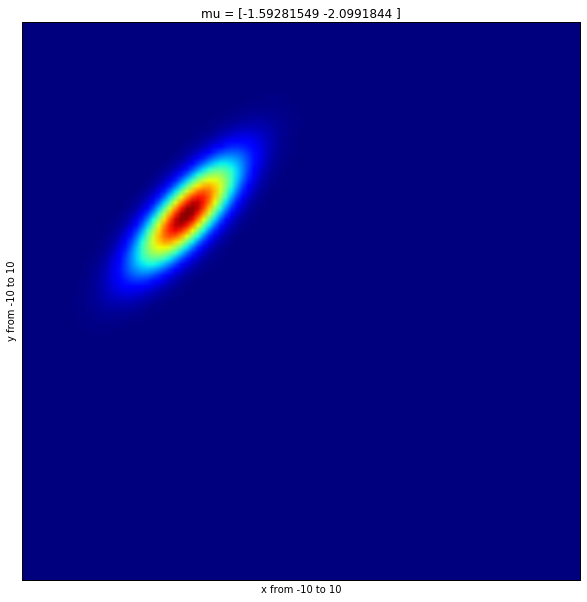
\includegraphics[scale = .5]{posterior.png}
	\end{center}
	
	Here is the code:
	\lstinputlisting[language=Python]{logistic_posterior.py}

\end{solution}

\newpage

\textbf{3 (Monte-Carlo Predictive Posterior)} From Problem 2 we have the distribution
$\PP(\ww|\Dc)$. Now suppose we want to compute the probability that a test point $\xx$
belongs to class $1$. Analytically, we marginalize out $\ww$ as
\[
    \PP(\yy=1|\xx,\Dc) = \int \PP(\yy=1|\xx,\ww)\PP(\ww|\Dc)~d\ww.
\]
Unfortunately, this integral cannot be computed in closed form (we say the integral is
intractable). On the other hand, a Simple Monte Carlo approximation of the integral is
\begin{align*}
    \PP(\yy=1|\xx,\Dc) \approx \frac{1}{S}\sum_{s=1}^S \PP(\yy=1|\xx,\ww^{(s)}).\tag{$\ww^{(s)}\sim\PP(\ww|\Dc)$}
\end{align*}
This is an unbiased estimate of the true predictive probability in the sense that its expectation
is $\PP(\yy=1|\xx,\Dc)$. This is also easy to compute since we approximated $\PP(\ww|\Dc)$ as
a Gaussian, so we can sample from it easily.
\begin{enumerate}[(a)]
    \item Given a function $f(\xx)$ where $\xx\sim \PP(\xx)$, show that
        \begin{align*}
            \EE_{\PP(\{\xx^{(s)}\})}[\hat f] = \EE\left[\frac{1}{S}\sum_{s=1}^S f(\xx^{(s)})\right] = \EE[f(\xx)].\tag{$\xx^{(s)}\sim\PP(\xx)$}
        \end{align*}
        Put in other terms, show that our Monte Carlo estimator is unbiased.
    \item Show that the variance of the Monte Carlo estimate is proportional to
        $1/S$. That is, show
        \begin{align*}
            \mathbb{V}_{\PP(\{\xx^{(s)}\})}[\hat f] = \mathbb{V}[f(\xx)]/S.
        \end{align*}
        Note that this means that standard deviation error bars shrink like $1/\sqrt{S}$.
    \item Plot the posterior predictive distribution $\PP(\yy=1|\xx,\Dc)$ overlaying your data
        using this Monte Carlo approximation. You plot should look similar to Figure 8.6 in
        Murphy.
\end{enumerate}

\begin{solution}
	\begin{enumerate}[(a)]
		\item 
			The definition of the dicrete expected value is
			\begin{align*}
				& \EE \left[\frac1S \sum_{s=1}^S f(\xx^{(s)}) \right] \\
				&= \frac1S \sum_{s=1}^S \EE [f(\xx^{(s)})] \\
				&= \frac1S \sum_{s=1}^S \EE [f(\xx)] \text{ Because distributed the same} \\
				&= \frac{S}{S} \EE [f(\xx)] \text{ As desired}
			\end{align*}
		\item
			The variance is 
			\begin{align*}
				\EE \left[ \left(\frac1S \sum_{s=1}^S f(\xx^{(s)})\right)^2 \right]- \EE \left[\frac1S \sum_{s=1}^S f(\xx^{(s)}) \right]^2
				&\propto \frac{1}{S^2} \text{ Because $\EE$ is linear operator.}
			\end{align*}
			Which is proportional to $\frac1S$ once we multiply by $S$.

		\item
			From the code in problem 2:\\\\
			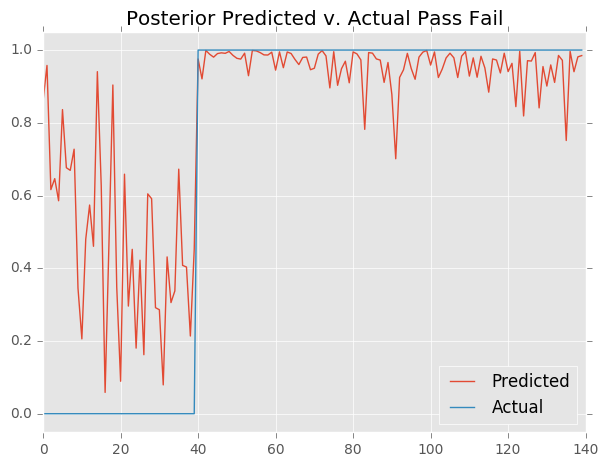
\includegraphics[scale = 1]{pred.png}
	\end{enumerate}
\end{solution}

\end{document}